\section{Description}

While statistical alignment is typically performed using pairwise hidden Markov
models, finite-state transducers (FSTs) \green{present themselves as a better
alternative}.
% too brief?
FSTs \green{also} have the ability to rigorously model molecular sequence
evolution in addition to well established methods for combining them in
different ways \parencite{bradley2007transducers}.
A powerful and versatile algorithm is composition, which consists of sending the
output of one FST as the input of a second FST.
The FST model implemented in COATi is designed by composing smaller FSTs, each
representing a specific process.

% Evolution FST
Pairwise alignment in COATi is implemented via the Evolution FST (Fig.
\ref{fig:evolution-fst}), based on existing transducers (e.g.
\cite{holmes2001evolutionary}).
The Evolution FST is formed by composing a substitution FST that encodes a 64x64
codon model and an indel FST that models insertions and deletions, including
frameshifts.
The innovation of the Evolution FST with respect to other transducers is the
combination of a codon substitution model with gaps that can occur at any
position of any length.

\begin{figure}[h!]
\begin{framed}
\centering
    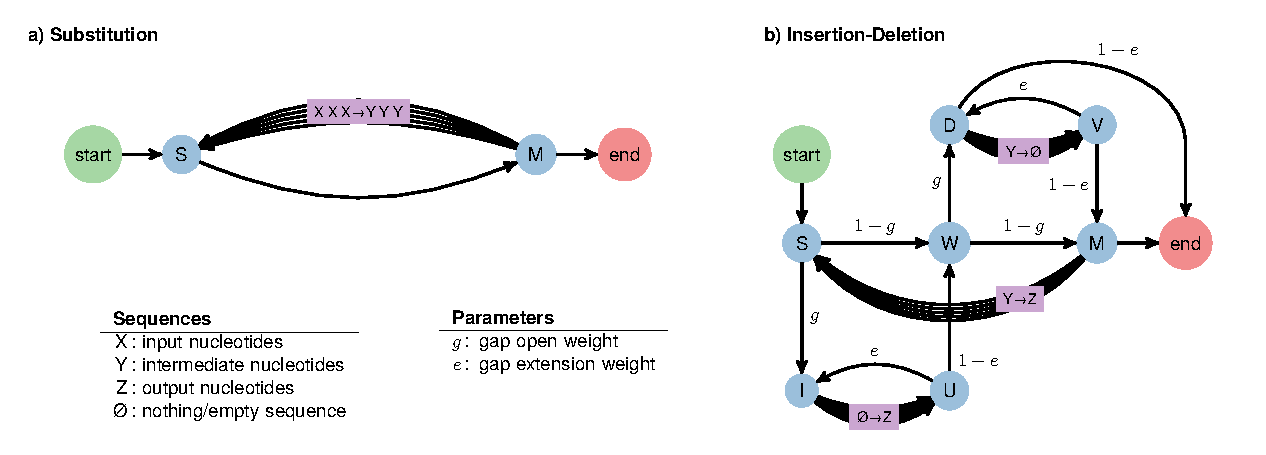
\includegraphics[width=\textwidth]{fig-evolution-fst.pdf}
    \caption{The evolution FST is assembled by composing a substitution FST and
    an indel FST. Each node represents a state in an FST while arcs display
    possible transitions between states (and their weights). Absorption and
    emission of symbols occurs between states. (a) The substitution FST
    encodes a 64x64 codon substitution model with 64 arcs from M to S. (b)
    The indel FST allows for insertions (I to U) and deletions (D to V).
    Contiguous insertions and deletions are always arranged for insertions to
    precede deletions to limit equivalent alignments.}
    \label{fig:evolution-fst}
\end{framed}
\end{figure}


% FST implementation
The alignment FST is the result from composing both sequences with the Evolution
FST.
Any path through the alignment FST represents a pairwise alignment, while the
shortest path corresponds to the best alignment.
% A path through the FST that \green{results} from composing both sequences with
% the Evolution FST represents a pairwise alignment.
% The shortest path through the FST corresponds with the best alignment.
However, composing large FSTs is expensive and can be prohibitive \green{(specify
I talk about time)}.
Despite the existence of efficient C++ FST libraries (e.g. openFST
\cite{allauzen2007openfst}), runtime is still limiting for sequence longer than
a few thousand nucleotides.
\green{To solve this issue, the search for an optimal path (alignment)} can be
reformulated as a dynamic programming problem.
